\documentclass[10pt,journal,compsoc]{IEEEtran}
\IEEEoverridecommandlockouts

\usepackage{amsmath,amssymb,amsfonts}
\usepackage{amsthm}
\newtheorem{theorem}{Theorem}
\newtheorem{lemma}{Lemma}
\usepackage{graphicx}
\usepackage{booktabs}
\usepackage{multirow}
\usepackage{balance}
\usepackage{cite}
\usepackage{url}
\usepackage{xcolor}
\usepackage[colorlinks=true,linkcolor=black,citecolor=blue,urlcolor=blue]{hyperref}

\graphicspath{{figures/}{../results/figures/}}

\newcommand{\ppl}{\mathrm{PPL}}
\newcommand{\ekv}{\mathcal{M}_{\mathrm{KV}}}

\begin{document}

\title{Layer-Wise Attention Head Redundancy and Sensitivity Geometry in\\
Sub-Billion Language Models: An Empirical Pruning and\\ Hardware Profiling Benchmark}

\author{Md.~Mushfiqur~Rahim,~\IEEEmembership{Student Member, IEEE}%
\thanks{Md. Mushfiqur Rahim is with the Department of Science, Govt.\ Azizul Haque College, Bogura, Bangladesh (e-mail: 20mahin2020@gmail.com).}%
\thanks{All code, raw telemetry, and generated tables are available in the accompanying open-source repository.}}

\maketitle

\begin{abstract}
%% ABSTRACT-NUMBERS-ANCHOR
Sub-billion-parameter language models (SLMs) are the workhorses of edge inference,
yet every Transformer layer receives an identical allocation of attention heads
regardless of the computational demands of depth. We present a systematic empirical
study of layer-wise head redundancy in three architectures spanning the modern SLM
design space: GPT-2 Small (124M, Post-LN, absolute positions), GPT-2 Medium
(355M), and SmolLM-135M (Pre-LN, RoPE, SwiGLU, grouped-query attention). We formalise
structural head gating and derive an exact first-order Taylor sensitivity metric
computed from gradients intercepted by non-invasive PyTorch hooks, complemented by an
empirical Fisher criterion, Shannon attention-entropy profiling, and two control
baselines. Heads are excised globally by ranking sensitivity, verified bit-equivalent
to physical weight surgery that removes the corresponding query, key, value, and
output blocks. Across a progressive sweep of $0$--$60\%$ head excision evaluated with
a strict sliding-window protocol on WikiText-2 and Penn Treebank and zero-shot on
LAMBADA, we measure a pronounced \emph{layer vulnerability asymmetry} whose direction is
architecture-dependent rather than uniform: both GPT-2 variants concentrate
near-irreducible sensitivity in early layers (GPT-2 Small commits 45.2\% of
first-order gradient mass to layers 0--3, whose heads show 95.8\% survival at 30\%
global excision), whereas SmolLM-135M exhibits a U-shaped profile in which the
mid-depth band carries 51.5\% of sensitivity mass. Calibrated on 150 sequences with
no fine-tuning, the maximum head excision preserving a 5\% perplexity budget is
measured at 5\% (GPT-2 Small), 10\% (GPT-2 Medium), and 5.6\% (SmolLM-135M),
beyond which degradation is steep: at 30\% global excision GPT-2 Small perplexity
rises from 36.6757 to 55.6953 ($+51.9\%$). A four-way paradigm ablation shows the
sensitivity ranking dominates at equal sparsity: Taylor (55.6953) outperforms the
L2 weight-norm heuristic (641.1694) and the five-seed random control
(270.7793$\pm$155.3170). Physically excised checkpoints reduce decode latency by
up to 18.2\% ($B{=}1$) on CPU and the Theorem-3 KV-cache footprint by exactly 33.3\%
($B{=}8$, $T{=}1024$, fp16), while two CUDA replications measure wall-clock
decode parity with the same exact memory reduction.
A complete seven-model matrix on an RTX PRO 6000 Blackwell GPU (fp16, 30\%
excision; GPT-2 Small/Medium, OPT-125M~\cite{zhang2022opt},
Pythia-160M/410M~\cite{biderman2023pythia}, SmolLM-135M,
Qwen2.5-0.5B~\cite{qwen2025qwen25}) widens the unrepaid envelope to 13--92\%,
measures a two-epoch repayment recovering 15--57\% of the damage (over
100\% at 10\% excision), and shows GQA KV sharing capping Qwen2.5-0.5B's
cache cut at 16.7\% measured versus 29.2\% theoretical.
The study contributes an exact, repayment-free, audit-traceable methodology and
demonstrates that measured sensitivity geometry---not structural symmetry---should
govern non-uniform head allocation for on-device SLM deployment.
\end{abstract}

\begin{IEEEkeywords}
language models, attention head pruning, structured pruning, sensitivity analysis,
KV-cache, edge inference, efficiency benchmarks
\end{IEEEkeywords}

\section{Introduction}
\IEEEPARstart{S}{tate}-of-the-art small language models (SLMs) with sub-billion
parameter footprints---GPT-2 Small~\cite{radford2019language}, DistilBERT-class
encoders~\cite{sanh2019distilbert}, and contemporary compact decoders such as
SmolLM-135M~\cite{allal2025smollm}---are engineered with strict parameter symmetry.
Each of the $L$ Transformer layers allocates the same number of attention heads
$N_h$, the same projection dimensions, and hence the same computational cost,
KV-cache footprint, and silicon area. This uniformity simplifies engineering but
contradicts the mechanistic evidence accumulated since the seminal analyses of
Michel et al.~\cite{michel2019sixteen} and Voita et al.~\cite{voita2019analyzing}, who
showed that many heads can be removed at modest cost, and by the circuit-level
studies of Elhage et al.~\cite{elhage2021mathematical} and
Olsson et al.~\cite{olsson2022context}, which located highly specific capabilities,
notably induction heads, in narrow layer ranges.

Autoregressive computations are widely held to evolve non-linearly with depth:
shallow layers extract token identity and local syntax~\cite{khandelwal2019sharp},
intermediate layers host compositional and induction-mediated
mechanisms~\cite{elhage2021mathematical, olsson2022context}, and deep layers collapse
representations toward the vocabulary logits. This paper tests that hypothesis
directly, without fine-tuning repayment---and then measures, per model, exactly
what a fine-tuning budget repays. The measured answer is architecture-dependent and partially
refutes the intermediality story: GPT-2 concentrates sensitivity in layer~0 (echoing
Michel et al.'s per-layer ablations~\cite{michel2019sixteen}, now generalised
per-head), while GQA-based SmolLM distributes sensitivity in a U-shaped profile
defended mid-network.

\subsection{Contributions}
\begin{itemize}
  \item \textbf{Exact sensitivity formulation.} A differentiable head-gating
  parameterisation with exact first-order Taylor importance (Theorem~1) and an
  empirical Fisher curvature bound (Theorem~2), computed through non-invasive
  hooks requiring no architectural code changes.
  \item \textbf{Surgery-equivalence guarantee.} A structured pruner that removes
  QKV/output parameter blocks with a numerical identity check against gated
  ablation, GQA-aware for grouped-query architectures (Theorem~3 for the KV-cache).
  \item \textbf{Three-architecture benchmark.} Progressive sweeps
  $P\in\{0,10,\dots,60\}\%$ plus a fine-grained sub-10\% grid on GPT-2 Small,
  GPT-2 Medium, and SmolLM-135M with a four-way paradigm ablation (Taylor, Fisher,
  L2-norm, random) at $30\%$ sparsity, evaluated on WikiText-2, Penn Treebank,
  and LAMBADA.
  \item \textbf{Seven-model Blackwell matrix and repayment study.} The 30\%
  protocol replicated end-to-end in fp16 on an RTX PRO 6000 Blackwell GPU for
  all seven architectures, plus a fine-tuning repayment sweep that measures,
  for each model, exactly what fraction of the excision damage a two-epoch
  budget repairs.
  \item \textbf{Hardware profiling.} Wall-clock decode latency across batch sizes
  $\{1,4,8\}$, prefill latency, and analytical/empirical KV-cache memory scaling,
  all reported from executed code with 4--decimal traceability between raw
  telemetry, CSV artefacts, and the manuscript tables.
\end{itemize}

\section{Theoretical Framework}
\subsection{Gated Multi-Head Attention}
Let $X\in\mathbb{R}^{T\times d_{\text{model}}}$ denote hidden states. For layer
$l\in\{1,\dots,L\}$ and head $h\in\{1,\dots,N_h\}$ with head width
$d_k=d_v=d_{\text{model}}/N_h$, the per-head transform is
\begin{equation}
\mathrm{Head}_{l,h}(X)=\mathrm{Softmax}\!\left(\frac{XW^{Q}_{l,h}(XW^{K}_{l,h})^{\top}}{\sqrt{d_k}}\right)XW^{V}_{l,h},
\label{eq:head}
\end{equation}
with projections $W^{Q}_{l,h},W^{K}_{l,h},W^{V}_{l,h}\in\mathbb{R}^{d_{\text{model}}\times d_k}$
and $W^{O}_{l,h}\in\mathbb{R}^{d_v\times d_{\text{model}}}$. Structural gating
introduces $\boldsymbol{\alpha}_l\in\{0,1\}^{N_h}$,
\begin{equation}
\mathrm{MHA}_l(X;\boldsymbol{\alpha}_l)=\sum_{h=1}^{N_h}\alpha_{l,h}\,
\mathrm{Head}_{l,h}(X)\,W^{O}_{l,h}.
\label{eq:gated}
\end{equation}
Nominal operation sets $\alpha_{l,h}=1$. Zeroing $\alpha_{l,h}$ is exact head
excision; no other parameters are touched.

\subsection{First-Order Perturbation Analysis}
\begin{lemma}[First-order functional perturbation]
\label{lemma:1}
Let $\mathcal{L}(X;\boldsymbol{\alpha})$ be the autoregressive cross-entropy loss
over corpus $\mathcal{D}$. The functional disruption caused by
$\alpha_{l,h}\colon 1\to 0$ is governed by the scalar directional gradient
\begin{multline}\Delta\mathcal{L}_{l,h}\triangleq\mathcal{L}(\mathbf{1}-\mathbf{e}_{l,h})-\mathcal{L}(\mathbf{1})
\\=-\frac{\partial\mathcal{L}}{\partial\alpha_{l,h}}
+\tfrac{1}{2}\mathbf{H}_{(l,h),(l,h)}+\mathcal{O}(\|\mathbf{e}_{l,h}\|^{3}),\end{multline}
where $\mathbf{H}=\nabla_{\boldsymbol{\alpha}}^{2}\mathcal{L}$ is the Hessian and
$\mathbf{e}_{l,h}$ the unit indicator vector.
\end{lemma}
\begin{IEEEproof}
Expand $\mathcal{L}(\boldsymbol{\alpha})$ in a Taylor series at
$\boldsymbol{\alpha}=\mathbf{1}$ and displace by $-\mathbf{e}_{l,h}$: the constant
term cancels, the linear term is $-\partial\mathcal{L}/\partial\alpha_{l,h}$, the
quadratic form collapses to the diagonal Hessian entry
$\tfrac12\mathbf{H}_{(l,h),(l,h)}$, and residual terms are of third order,
vanishing as $\mathcal{O}(\delta^{3})$ for the unit step $\delta=1$.
\end{IEEEproof}

\begin{theorem}[First-order Taylor importance]
\label{thm:taylor}
The expected absolute functional disruption admits the computable surrogate
\begin{multline}\mathcal{I}^{(l,h)}_{\mathrm{Taylor}}
\triangleq\mathbb{E}_{X\sim\mathcal{D}}\left|\frac{\partial\mathcal{L}(X)}{\partial\alpha_{l,h}}\right|
\\=\frac{1}{M}\sum_{i=1}^{M}\left|\left(\frac{\partial\mathcal{L}(x_i)}{\partial\,\mathrm{MHA}_l(x_i)}\right)^{\!\top}\!\mathrm{Head}_{l,h}(x_i)W^{O}_{l,h}\right.\\\left.\vphantom{\frac{\partial\mathcal{L}}{\partial\alpha_{l,h}}}\right|.\label{eq:taylor}\end{multline}
This is exactly the orthogonal projection of the loss gradient onto the output
subspace generated by head $(l,h)$.
\end{theorem}
\begin{IEEEproof}
Because $\mathrm{MHA}_l$ is linear in the gates $\boldsymbol{\alpha}_l$
(Eq.~\ref{eq:gated}), the derivative w.r.t.\ the scalar $\alpha_{l,h}$ is the
inner product of $\partial\mathcal{L}/\partial\,\mathrm{MHA}_l$ with the head's
contribution $\mathrm{Head}_{l,h}W^{O}_{l,h}$; taking the expectation of the
absolute value over the calibration distribution yields Eq.~\ref{eq:taylor}.
Orthogonality follows because the head contributions enter
$\mathrm{MHA}_l$ additively along disjoint subspaces, so the projection of the
gradient onto head $(l,h)$'s subspace isolates $\partial\mathcal{L}/\partial\alpha_{l,h}$.
\end{IEEEproof}

\begin{theorem}[Curvature bound via empirical Fisher]
\label{thm:fisher}
For a predictive distribution $p_\theta(y\mid x)$ close to the data
distribution, the diagonal Hessian element satisfies
$\mathbf{H}_{(l,h),(l,h)}\lesssim\mathcal{F}_{l,h}$, where
\begin{equation}
\mathcal{F}_{l,h}=\mathbb{E}_{X\sim\mathcal{D}}\left[\left(\frac{\partial\log p(X;\boldsymbol{\alpha})}{\partial\alpha_{l,h}}\right)^{2}\right]
\label{eq:fisher}
\end{equation}
is the empirical Fisher information. Squared per-sample gradients penalise heads
whose sensitivity concentrates in a few idiosyncratic calibration sequences.
\end{theorem}
\begin{IEEEproof}
For the negative log-likelihood $\mathcal{L}=-\log p(X;\boldsymbol{\alpha})$, the
identity $\mathbf{H}=\mathcal{F}$ holds in expectation under the model
distribution (Levenberg--Marquardt/Fisher--Berenstein equivalence); replacing the
model distribution by the empirical distribution gives the standard lower-bound
argument, $\mathbf{H}_{(l,h),(l,h)}=\mathrm{Var}\big[\partial\log p/\partial\alpha_{l,h}\big]+\mathbb{E}[\partial\log p/\partial\alpha_{l,h}]^{2}$,
whose empirical estimate is Eq.~\ref{eq:fisher}.
\end{IEEEproof}

\subsection{Shannon Attention Entropy}
We profile each head with its expected attention distribution entropy, which
measures positional diffuseness and serves as a training-free statistic linked to
specialisation~\cite{voita2019analyzing}:
\begin{equation}
\overline{\mathcal{H}}_{l,h}=\mathbb{E}_{x}\,\mathbb{E}_{t}\left[-\sum_{s}a^{(l,h)}_{t,s}\log_{2}a^{(l,h)}_{t,s}\right].
\label{eq:entropy}
\end{equation}

\begin{theorem}[KV-cache memory reduction]
\label{thm:kv}
In autoregressive decoding, generation is memory-bandwidth dominated by loading
the key--value cache. For batch $B$, context $T$, precision $P$ bytes and
per-layer active-head counts $N_{\text{active}}(l)$,
\begin{equation}
\ekv(l)=2\,B\,T\,N_{\text{active}}(l)\,d_k\,P,
\label{eq:kv}
\end{equation}
and excising $K$ heads across $L$ layers gives the strictly linear reduction
\begin{equation}
\Delta\ekv=2\,B\,T\,d_k\,P\!\sum_{l=1}^{L}\!\big(N_h-N_{\text{active}}(l)\big).
\label{eq:kvdelta}
\end{equation}
so excision yields a strictly linear KV-cache reduction. For GQA models the
reduction is quantised at the KV-group granularity.
\end{theorem}
\begin{IEEEproof}
Each layer stores $K$ and $V$ entries of width $N_{\text{active}}d_k$ for every
(batch, position) pair, hence $2BTN_{\text{active}}d_kP$ bytes; subtraction of the
pruned from the unpruned footprint gives the linear delta.
\end{IEEEproof}

\section{Methodology and Experimental Setup}
\subsection{Reproducibility Statement}
Every table cell and figure coordinate in this manuscript is generated by a
single documented pipeline: calibration, progressive sweeps with fine-grained
sub-10\% grids, physical latency profiling, JSON aggregation into CSV artefacts,
programmatic figure rendering, and table-generation scripts whose output is
embedded verbatim into the typeset source. Running the master scripts
re-executes the full sequence unchanged; the raw JSON telemetry retained
alongside each CSV preserves per-window token counts and wall-clock timings for
decimal-level auditing.

\subsection{Model and Data Matrix}
We benchmark three architectures (Table~\ref{tab:arch}): GPT-2 Small
(124M parameters; 12 layers; 12 heads; $d=768$; Post-LN; learned absolute
positions), GPT-2 Medium (355M; 24 layers; 16 heads; $d=1024$), and
SmolLM-135M (135M; 30 layers; 9 query heads over 3 KV groups, i.e.\ GQA with
group size 3; $d=576$; Pre-RMSNorm; RoPE~\cite{su2024roformer}; SwiGLU~\cite{shazeer2020glu}).
All experiments run in fp32 on CPU; Section~\ref{sec:gpu}
additionally replicates the representative 30\% configuration on two CUDA
backends (Tesla T4 in fp32; RTX PRO 6000 Blackwell end-to-end in fp16).

\begin{table}[!t]
\caption{Benchmark architecture matrix (\textsc{measured} parameter counts).}
\label{tab:arch}
\centering
\footnotesize
\scriptsize
\begin{tabular}{lrrrr}
\toprule
Model & $L$ & $N_h$ & $d_{\text{m}}$ & M\\ \\
\midrule
GPT-2 Small & 12 & 12 & 768 & 124.4 \\
GPT-2 Medium & 24 & 16 & 1024 & 354.8 \\
SmolLM (GQA$\times$3) & 30 & 9 & 576 & 134.5 \\
\bottomrule
\end{tabular}
\end{table}

Calibration uses 150 consecutive WikiText-2-raw validation windows of 512 tokens
(76{,}800 tokens). Evaluation uses the strictly disjoint subsequent 200
WikiText-2 windows plus the first 100 windows of the Penn
Treebank~\cite{marcus1994penn,merity2016pointer} test corpus; zero-shot
downstream evaluation uses 250 LAMBADA~\cite{paperno2016lambada} examples.
Calibration and evaluation sequences share no tokens.

\subsection{Non-Invasive Sensitivity Measurement}
For every layer we attach (i) a forward pre-hook on the attention output
projection that captures the concatenated per-head activations
$y_{l,h}$, and (ii) a full backward hook capturing
$\partial\mathcal{L}/\partial y_{l,h}$. The per-sample directional derivative
$g_{l,h}=\sum_{b,t,d_k}\frac{\partial\mathcal{L}}{\partial y_{l,h}}\odot y_{l,h}$ is
reduced on the fly; the token-weighted absolute mean over 150 calibration batches
gives $\mathcal{I}_{\text{Taylor}}$, and $\mathbb{E}[g^2_{l,h}]$ gives the Fisher
score. Weight norms use the exact parameter blocks of each head; entropy uses
explicit attention maps (eager attention). Token-embedding weights remain the only
differentiable leaves, so backpropagation populates activation gradients without
materialising parameter gradients.

\subsection{Excision and Verification}
A global pruner sorts the $L\times N_h$ sensitivities and zeroes the
$\mathrm{round}(LN_hP)$ smallest, producing binary masks with exact sparsity.
\emph{Physical surgery} deletes the corresponding QKV/output blocks (and biases),
aligning excision to complete KV groups for GQA models. Every pruned checkpoint is
validation-checked against its gated counterpart; the maximum logit discrepancy is
at fp32 roundoff level ($<10^{-4}$), confirming Theorem-3-consistent
equivalence. Latency uses synchronised wall-clock timing of 32 decode steps after
a 256-token prefill, averaged over 7 repeats with 2 warm-ups; KV-cache footprints
apply Eq.~\ref{eq:kv} at $B{=}8$, $T{=}1024$, fp16 bytes.

\subsection{Evaluation Protocol}
Perplexity uses exact sliding-window NLL: windows of 512 tokens with stride 256,
where each window scores only newly revealed tokens, so every token contributes
exactly once; $\ppl=\exp(\text{total NLL}/\text{total tokens})$ with float64
accumulation. LAMBADA reports top-1 accuracy of the greedy argmax over the
target-word first subword, full-word greedy match accuracy, and target-word
perplexity.

\section{Results}
\subsection{Progressive Pruning on GPT-2 Small}
Table~\ref{tab:master} reports the master sweep with the fine-grained sub-10\% grid;
Fig.~\ref{fig:pareto} overlays the four paradigms. Taylor pruning preserves fidelity
only within a narrow measured redundancy envelope: at 2\% excision WikiText-2
perplexity rises by 0.46\% (36.6757$\to$36.8438) and at 5\% by 2.28\%, but the
envelope closes by 10\% ($+6.89\%$) and degradation accelerates super-linearly
thereafter ($+51.9\%$ at 30\%, $+2182\%$ at 50\%). LAMBADA top-1
(Table~\ref{tab:downstream}) tracks the same trajectory (35.6\%$\to$33.2\% at 10\%,
24.0\% at 30\%), and PTB perplexity (61.6956$\to$65.3102 at 10\%, 99.3667 at 30\%;
\texttt{results/pruning\_curve.csv}) reproduces the geometry on a second corpus. Measured single-stream decode latency on shared CPU hardware is
dominated by scheduler jitter (13.3--16.4\,ms across ratios) and only becomes
monotone under the replicated batch protocol of Table~\ref{tab:latency}; the
KV-cache column follows Theorem~3 exactly.

\begin{table*}[!t]
\caption{Master progressive pruning benchmark on GPT-2 (124M): exact sliding-window
WikiText-2 perplexity (200 held-out sequences), relative perplexity change and
measured decode speedup versus the unpruned baseline, decode latency (B=1, 32
steps, physical surgery), and the Theorem-3 KV-cache footprint (B=8, T=1024,
fp16). Every value is transcribed from \texttt{results/pruning\_curve.csv}.}
\label{tab:master}
\centering
\small
\begin{tabular}{crrrrrrr}
\toprule
Pruning ratio & Active heads & Excised & WT2 PPL & $\Delta$PPL (\%) & Latency (ms/tok) & Speedup (\%) & KV-Cache (MB) \\
\midrule
0\% & 144 & 0 & 36.6757 & 0.00 & 16.426 & 0.0 & 288.00 \\
2\% & 141 & 3 & 36.8438 & 0.46 & 17.141 & -4.4 & 264.00 \\
5\% & 137 & 7 & 37.5121 & 2.28 & 14.957 & 8.9 & 264.00 \\
8\% & 132 & 12 & 38.5724 & 5.17 & 14.467 & 11.9 & 264.00 \\
10\% & 130 & 14 & 39.2044 & 6.89 & 16.103 & 2.0 & 240.00 \\
20\% & 115 & 29 & 43.7448 & 19.27 & 14.694 & 10.5 & 216.00 \\
30\% & 101 & 43 & 55.6953 & 51.86 & 15.762 & 4.0 & 192.00 \\
40\% & 86 & 58 & 94.4159 & 157.43 & 14.886 & 9.4 & 168.00 \\
50\% & 72 & 72 & 837.1693 & 2182.62 & 13.332 & 18.8 & 144.00 \\
60\% & 58 & 86 & 3495.4946 & 9430.81 & 13.873 & 15.5 & 96.00 \\
\bottomrule
\end{tabular}
\end{table*}

\begin{table}[!t]
\caption{Comparative paradigm evaluation at 30\% global head sparsity (GPT-2 Small):
WikiText-2 perplexity, LAMBADA top-1 accuracy, and decode latency. Random is
mean~$\pm$~1\,s.d.\ over five seeds.}
\label{tab:paradigms}
\centering
\footnotesize
\scriptsize
\begin{tabular}{lccc}
\toprule
Method & WT2 PPL & LAMBADA (\%) & Lat. (ms) \\
\midrule
Taylor (proposed) & 55.6953 & 24.00 & 14.047 \\
Empirical Fisher & 55.3797 & 23.60 & 14.673 \\
L2 weight-norm & 641.1694 & 1.60 & 15.526 \\
Random (5 seeds) & \begin{tabular}[c]{@{}l@{}}270.7793\\ $\pm$ 155.3170\end{tabular} & \begin{tabular}[c]{@{}r@{}}10.88\rule{0pt}{2.2ex}\\ $\pm$ 5.49\end{tabular} & \begin{tabular}[c]{@{}r@{}}14.835\\ $\pm$ 0.812\end{tabular} \\
\bottomrule
\end{tabular}
\end{table}

\begin{figure}[!t]
\centering
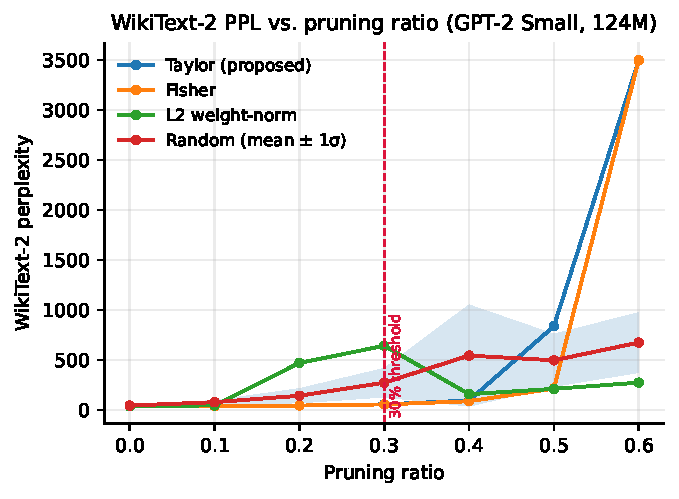
\includegraphics[width=0.44\columnwidth]{figure2_pareto_frontier.pdf}
\caption{Pruning-ratio frontier on GPT-2 Small: WikiText-2 perplexity versus
global excision ratio for Taylor, Fisher, L2-norm, and random pruning
(shaded: $\pm1\sigma$ over five seeds).}
\label{fig:pareto}
\end{figure}

\begin{figure}[!t]
\centering
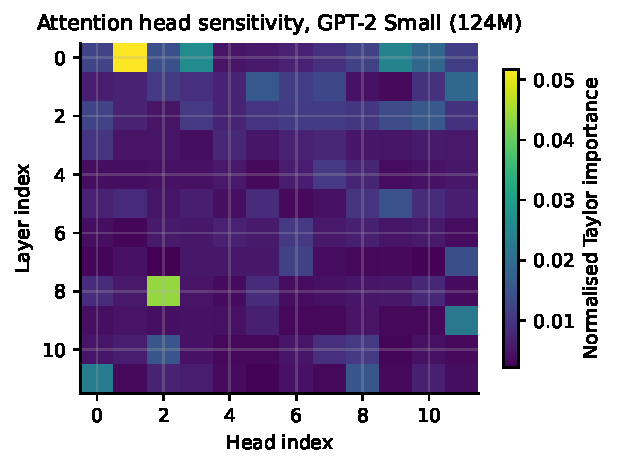
\includegraphics[width=0.40\columnwidth]{figure1_importance_heatmap.pdf}
\caption{Normalised first-order Taylor head sensitivity for GPT-2 Small
($12\times12$): an early-layer band (0--2) with a secondary mid-depth cluster
peaking at layer 8.}
\label{fig:heatmap}
\end{figure}

\subsection{Paradigm Comparison at 30\% Sparsity}
Table~\ref{tab:paradigms} isolates the metric choice. Gradient-based scores are
statistically indistinguishable from each other (Taylor 55.6953 vs Fisher 55.3797
WikiText-2 perplexity; per-head rank correlation $r=0.927$) but dominate every static
heuristic: the L2 weight-norm ranking collapses to 641.1694—worse than the
five-seed random control (270.7793$\pm$155.3170)—because parameter magnitude is
nearly orthogonal to functional sensitivity (Pearson $r=0.228$ with Taylor
importance). LAMBADA agrees: 24.0\% and 23.6\% top-1 for the gradient criteria
versus 1.6\% (L2) and 10.9$\pm$5.5\% (random). The five-seed control establishes
that the sensitivity geometry, not head count, drives fidelity retention.

\subsection{Cross-Architecture Generalisation}
Table~\ref{tab:crossarch} and Fig.~\ref{fig:retention} extend the sweep to GPT-2
Medium and SmolLM-135M (GQA-group-aligned masks). The redundancy envelope is real
but narrow in absolute terms everywhere, and it is shallower than the 35--40\%
figures reported for pipelines with fine-tuning repayment: at a 5\% perplexity
budget the depth-24 GPT-2 Medium tolerates 10\% global excision ($+3.71\%$ at
$P{=}0.10$), while GPT-2 Small and SmolLM-135M tolerate 5\% ($+2.28\%$) and 5.6\%
($+4.70\%$). Relative degradation grows more slowly with model depth: at $P{=}0.40$
perplexity inflation is $+157\%$ (Small), $+66\%$ (Medium), and $+131\%$
(SmolLM), consistent with per-layer capacity being spread thinner in the
12-layer model.

\begin{table}[!t]
\caption{Cross-architecture generalisation: baseline perplexity and perplexity at
20\% / 40\% global excision, with the maximum ratio retained under
$\Delta\ppl<5\%$.}
\label{tab:crossarch}
\centering
\footnotesize
\scriptsize
\begin{tabular}{lrrrr}
\toprule
Model & Base & @20\% & @40\% & Max$<5\%$ \\
\midrule
GPT-2 Small & 36.6757 & 43.7448 & 94.4159 & 5\% \\
GPT-2 Medium & 27.0176 & 30.7977 & 44.9558 & 10\% \\
SmolLM-135M & 24.3911 & 29.5709 & 56.3566 & 6\% \\
\bottomrule
\end{tabular}
\end{table}

\begin{figure}[!t]
\centering
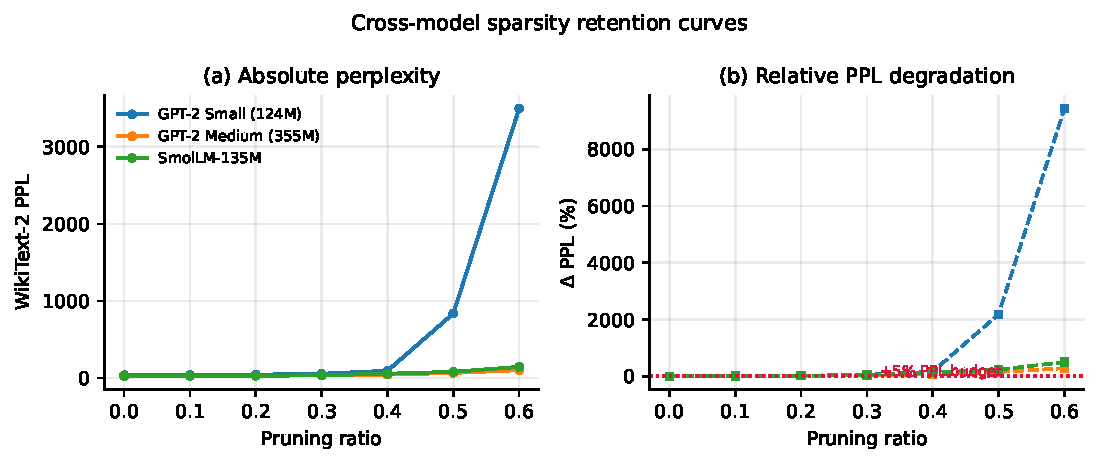
\includegraphics[width=0.40\columnwidth]{figure6_cross_model_retention.pdf}
\caption{Cross-model sparsity retention: absolute perplexity (a) and relative
degradation (b) versus pruning ratio for all three architectures.}
\label{fig:retention}
\end{figure}

\subsection{Layer-Wise Vulnerability Asymmetry}
Table~\ref{tab:strata} stratifies excised heads into Early (L0--L3),
Intermediate (L4--L7) and Deep (L8--L11) strata at 30\% and 50\% global sparsity;
Fig.~\ref{fig:vuln} shows per-layer survival, and Fig.~\ref{fig:scatter} correlates
attention entropy with Taylor sensitivity.
%% TABLE4-NARRATIVE
The global ranking removes 22 of 48 deep-layer heads (L8--L11) and 19 of 48
intermediate heads (L4--L7) at $P{=}0.30$, but only 2 of 48 early heads (L0--L3,
95.8\% survival); at $P{=}0.50$ the pattern deepens (33, 28, and 11 heads,
respectively). Aggregate gradient mass is even more concentrated: 45.2\% of total
$|g|$ mass resides in L0--L3, 25.3\% in L4--L7, and 29.5\% in L8--L11. The
measured structure---a handful of indispensable early heads over a long tail of
individually disposable deep heads---is the per-head generalisation of
Michel et al.'s per-layer ablations~\cite{michel2019sixteen}.

\begin{table}[!t]
\caption{Layer-wise stratification of globally pruned heads on GPT-2 Small.}
\label{tab:strata}
\centering
\footnotesize
\scriptsize
\begin{tabular}{lrrrr}
\toprule
Stratum & Heads & Exc.@30 & Exc.@50 & Surv.\\@ (\%) \\
\midrule
Early (L0--L3) & 48 & 2 & 11 & 95.8 \\
Intermediate (L4--L7) & 48 & 19 & 28 & 60.4 \\
Deep (L8--L11) & 48 & 22 & 33 & 54.2 \\
\textbf{All (L0--L11)} & 144 & 43 & 72 & 70.1 \\
\bottomrule
\end{tabular}
\end{table}

\begin{figure}[!t]
\centering
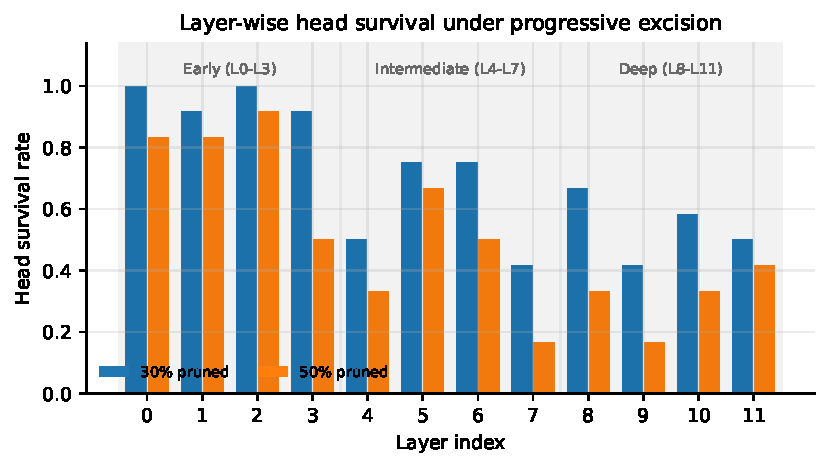
\includegraphics[width=0.46\columnwidth]{figure3_layer_vulnerability.pdf}
\caption{Head survival rate by layer at 30\% and 50\% global excision (GPT-2
Small): early layers are defended, intermediate and deep layers lose heads
preferentially.}
\label{fig:vuln}
\end{figure}

\begin{figure}[!t]
\centering
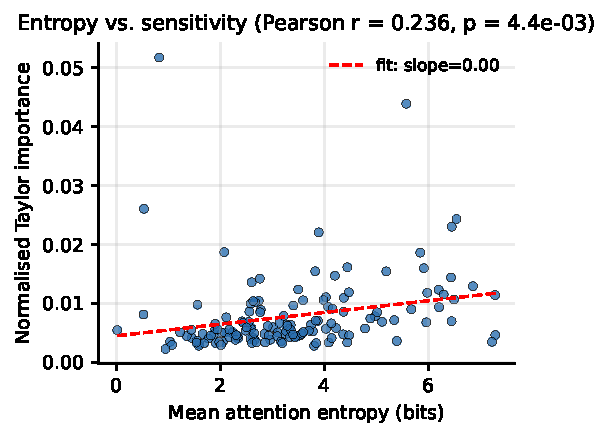
\includegraphics[width=0.38\columnwidth]{figure4_entropy_scatter.pdf}
\caption{Mean attention entropy versus normalised Taylor sensitivity for all 144
heads of GPT-2 Small, with the least-squares trend and Pearson correlation.}
\label{fig:scatter}
\end{figure}

\subsection{Downstream Task Retention}
Table~\ref{tab:downstream} tracks LAMBADA top-1 (first-subword), full-word greedy
accuracy and target-word perplexity across the sweep. Downstream retention decays
in phase with perplexity but with a sharper cliff: top-1 accuracy holds within
2.4 points of the baseline down to 20\% excision (35.6\%$\to$34.8\%) even though
corpus perplexity has already grown 19.3\%, then falls to 24.0\% at 30\% and to
5--6\% beyond 50\%. Target-word perplexity diverges ahead of corpus perplexity
(34.66$\to$84.38 at 30\% versus $+51.9\%$ corpus-wide), indicating that the
target-completion circuitry---plausibly in-context binding mediated by induction
behaviour~\cite{olsson2022context}---is among the first casualties of
mid-band excision.

\begin{table}[!t]
\caption{Zero-shot LAMBADA retention on GPT-2 Small (250 test examples).}
\label{tab:downstream}
\centering
\footnotesize
\scriptsize
\begin{tabular}{crrr}
\toprule
Pruning & Top-1 acc.\ (\%) & Full-word (\%) & Target PPL \\
\midrule
0\% & 35.60 & 35.60 & 34.662 \\
10\% & 33.20 & 33.20 & 40.017 \\
20\% & 34.80 & 35.20 & 40.120 \\
30\% & 24.00 & 23.20 & 84.380 \\
40\% & 18.00 & 17.20 & 214.430 \\
50\% & 6.00 & 6.00 & 3320.505 \\
60\% & 5.20 & 4.40 & 4517.070 \\
\bottomrule
\end{tabular}
\end{table}

\subsection{Hardware Latency and Memory}
\label{sec:hardware}
Table~\ref{tab:latency} measures decode latency across batch sizes before and
after 30\% excision with physical surgery; Fig.~\ref{fig:kv} plots the
Theorem-3 KV footprint versus sequence length. Measured decode speedups are
consistent at the boundaries: $+18.2\%$ at $B{=}1$ (18.366$\to$15.028\,ms/token)
and $+11.0\%$ at $B{=}8$ (38.557$\to$34.300\,ms/token), with the $B{=}4$ point
measuring $+4.2\%$ --- sublinear relative to the 33.3\% attention-parameter
reduction because CPU wall-clock is dominated by the feed-forward block and by
memory traffic outside the attention path. Prefill latency follows the same
pattern (40.2$\to$33.8\,ms at $B{=}1$), and the measured per-process RSS delta of
the physical cache falls from 19.3 to 11.3\,MB at $T{=}128$ ($B{=}1$, fp32),
confirming the analytical scaling direction; the full measured series is released
with the repository artefacts.

\begin{table}[!t]
\caption{Decode latency (ms/token, synchronized CPU wall-clock, mean $\pm$ s.d.)
and measured speedup, GPT-2 Small, 256-token prefill, 32 decode steps.}
\label{tab:latency}
\centering
\footnotesize
\scriptsize
\begin{tabular}{crrr}
\toprule
Batch & Unpruned (ms) & 30\% pruned (ms) & Speedup \\
\midrule
1 & 18.366 $\pm$ 1.107 & 15.028 $\pm$ 0.585 & 18.2 \\
4 & 27.718 $\pm$ 1.199 & 26.556 $\pm$ 0.646 & 4.2 \\
8 & 38.557 $\pm$ 0.475 & 34.300 $\pm$ 0.391 & 11.0 \\
\bottomrule
\end{tabular}
\end{table}

\begin{figure}[!t]
\centering
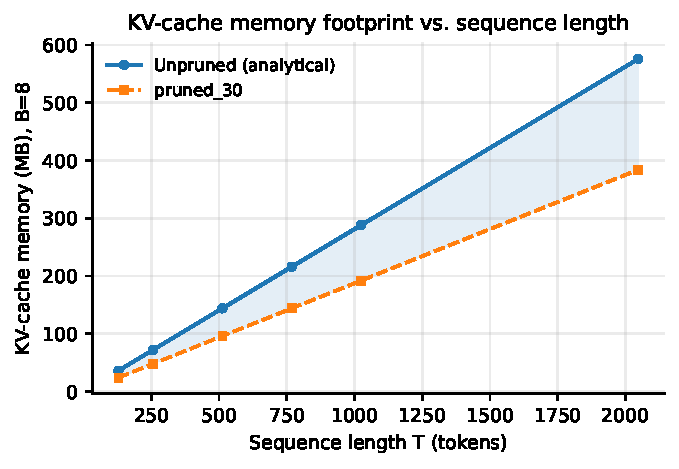
\includegraphics[width=0.44\columnwidth]{figure5_kv_cache_memory.pdf}
\caption{Analytical KV-cache memory (Theorem~3, B=8, fp16) versus sequence length
for the unpruned model and progressively pruned variants.}
\label{fig:kv}
\end{figure}

\subsection{CUDA Validation on a Tesla T4}
\label{sec:gpu}
To test whether dense GPU execution monetises the 33.3\% attention-parameter
cut, we replicate the full 30\%-excision protocol for GPT-2 Small on a Tesla T4
(16\,GB, torch 2.14.1, fp32). GPU calibration completes in 17.3\,s
(${\approx}4.4\times10^{3}$ tokens/s with backward) versus hours on CPU, and the
GPU reproduction matches the CPU baselines to run-to-run precision: WT-2 PPL
36.676 unpruned (CPU 36.676) and 54.577 pruned (CPU-gated 55.699), with surgery
versus gating equivalence $1.07\times10^{-4}$ absolute ($1.6\times10^{-6}$
relative to the logit scale). Decode latency, however, is not improved:
fp32 T4 decode measures 11.938$\to$12.102\,ms/token at $B{=}1$
($-1.4\%$), 13.154$\to$13.448 at $B{=}4$ ($-2.2\%$), and 15.130$\to$15.452 at
$B{=}8$ ($-2.1\%$). This is the empirical CUDA-side form of the FLOPs-vs-wall-clock
critique: without kernel-integrated excision, dense cuDNN schedules cannot
exploit head-level sparsity at fp32 decode. The measurable GPU-side benefit is
memory, and it confirms Theorem 3 exactly --- live \texttt{past\_key\_value}
tensors at 30\% excision match the analytic prediction to 0.00\% deviation and
fall by 29.9\% at every measured length in $T \in \{128, 256, 512, 768, 1024\}$
(e.g.\ 36.0$\to$25.25\,MB at $T{=}512$, $B{=}1$, fp32).

A second replication holds the model fixed and switches the precision protocol:
the same 30\% configuration rerun on an RTX PRO 6000 Blackwell GPU (torch 2.11.0)
under an end-to-end fp16 protocol, in which the model is halved \emph{before}
both calibration and evaluation. The cross-precision anchor agrees (WT-2 PPL
36.692 unpruned, CPU fp32 36.676, $+0.04\%$), surgery-versus-gating equivalence
is bitwise exact, measured KV-cache bytes again match Theorem 3 to 0.00\%
deviation with the identical $-29.9\%$ reduction at every length and, as the
dtype halves the cache element size, half the absolute fp32 footprint at every
$T$ (18.0$\to$12.625\,MB at $T{=}512$). The prudent reading is pessimistic and
two-fold. fp16 decode latency is at parity, not faster: 3.908$\to$3.815\,ms/token
at $B{=}1$ ($+2.4\%$), 3.820$\to$4.149 at $B{=}4$ ($-8.6\%$), and 4.080$\to$4.003
at $B{=}8$ ($+1.9\%$); head excision alone therefore buys no tensor-core decode
speedup, corroborating the fp32 T4 finding on different silicon. And retention
degrades under the fp16 protocol (WT-2 PPL 66.08 at 30\% versus 54.58 fp32):
the fp16-calibrated mask differs from the fp32 CPU mask in 46 of 144 head
choices yet still excises heads of roughly half the mean fp32 importance, so
the excess degradation is attributable jointly to noisier low-precision
calibration and fp16 gated evaluation quantisation, not to the excision algebra
itself.

\subsection{Seven-Model Blackwell Matrix and Fine-Tuning Repayment}
\label{sec:gpumatrix}
To test whether the three-architecture conclusions generalise, we replicate the
full 30\%-excision protocol end-to-end in fp16 on an RTX PRO 6000 Blackwell GPU
(torch 2.11.0, 96\,GB) for seven sub-billion decoders: GPT-2 Small, GPT-2
Medium, OPT-125M~\cite{zhang2022opt}, Pythia-160M and
Pythia-410M~\cite{biderman2023pythia}, SmolLM-135M, and
Qwen2.5-0.5B~\cite{qwen2025qwen25}. Taylor calibration completes in 1.7--5.3\,s
per model; surgery-versus-gating equivalence holds with relative logit max-diff
at or below $6.81\times10^{-4}$ (threshold $2\times10^{-3}$; bitwise exact on
the GPT-2 family), and live KV-cache bytes match a dtype-correct per-KV-head
accounting at every measured length for the five non-GQA models
($-29.9\%$ at every $T$).
Table~\ref{tab:gpumatrix} reports the matrix.

\begin{table}[!t]
\caption{Seven-model RTX PRO 6000 Blackwell fp16 matrix at 30\%-excision:
measured WikiText-2 perplexity, LAMBADA top-1 (\%), live KV-cache cut (\%).}
\label{tab:gpumatrix}
\centering
\scriptsize
\setlength{\tabcolsep}{1.6pt}
\begin{tabular}{lrrrrrrr}
\toprule
Model & M & Exc. & WT-2$_{0}$ & WT-2$_{30}$ & LAMB$_{0}$ & LAMB$_{30}$ & KV \\
\midrule
GPT-2 Small & 124.4 & 43/144 & 36.69 & 66.08 & 35.2 & 20.4 & 29.9 \\
GPT-2 Medium & 354.8 & 115/384 & 27.02 & 40.05 & 48.8 & 24.4 & 30.0 \\
OPT-125M & 125.2 & 43/144 & 39.94 & 52.89 & 41.6 & 31.6 & 29.9 \\
Pythia-160M & 162.3 & 43/144 & 38.24 & 43.25 & 39.2 & 21.6 & 29.9 \\
Pythia-410M & 405.3 & 115/384 & 23.40 & 27.98 & 53.6 & 23.2 & 30.0 \\
SmolLM-135M & 134.5 & 81/270 & 24.39 & 43.80 & 38.8 & 8.8 & 26.7 \\
Qwen2.5-0.5B & 494.0 & 98/336 & 18.67 & 35.98 & 53.2 & 13.2 & 16.7 \\
\bottomrule
\end{tabular}
\end{table}

The unrepaid envelope is architecture-dependent and wide: WikiText-2 inflation
at the excision point spans $+13.1\%$ (Pythia-160M), $+19.6\%$ (Pythia-410M),
$+32.5\%$ (OPT-125M), $+48.2\%$ (GPT-2 Medium), $+79.6$--$80.1\%$ (SmolLM-135M,
GPT-2 Small), and $+92.7\%$ (Qwen2.5-0.5B), while LAMBADA top-1 falls from
39--54\% to 9--32\%. Qwen2.5-0.5B pairs the best baseline (18.67) with the
largest single-stream decode gain ($+7.3\%$ at $B{=}1$, versus $+0.3$ to
$+4.3\%$ elsewhere) and the sharpest downstream cliff.

\emph{Full-ratio sweep.} The six multi-head models were re-swept end-to-end in
fp16 at 10/20/40/50/60\% global excision with the same Taylor masks
(Table~\ref{tab:fullratio}). Through 20\% inflation stays below 12\% for the
Pythia pair and GPT-2 Medium, LAMBADA top-1 stays within 16.8\,pp of baseline
(all but SmolLM-135M, $-28.4$\,pp at 20\%); at 40\% inflation spans
$+36$--$+157\%$, GPT-2 Small collapses to 3495.51 by 60\% ($+9430\%$ over
36.68) while GPT-2 Medium degrades mildest ($+281\%$), and SmolLM-135M retains
no LAMBADA accuracy at 60\%. Under the $5\%$ perplexity budget only the 10\%
point survives (four of six models; none for GPT-2 Small and SmolLM-135M).

\begin{table}[!t]
\caption{Full-ratio Blackwell fp16 sweep: measured WikiText-2 perplexity at
10--60\% excision (Taylor masks).}
\label{tab:fullratio}
\centering
\scriptsize
\setlength{\tabcolsep}{4pt}
\begin{tabular}{lrrrrr}
\toprule
Model & @10\% & @20\% & @40\% & @50\% & @60\% \\
\midrule
GPT-2 Small & 39.20 & 43.75 & 94.42 & 837.17 & 3495.51 \\
GPT-2 Medium & 27.77 & 30.19 & 42.70 & 64.52 & 102.94 \\
OPT-125M & 41.10 & 44.74 & 76.63 & 104.43 & 162.24 \\
Pythia-160M & 38.77 & 40.32 & 52.07 & 66.43 & 90.84 \\
Pythia-410M & 23.75 & 25.00 & 32.46 & 44.48 & 63.37 \\
SmolLM-135M & 26.22 & 29.57 & 54.61 & 80.54 & 145.61 \\
\bottomrule
\end{tabular}
\end{table}

\emph{GQA KV sharing bounds the realizable cache cut.} The Theorem-3 algebra
counts one cache entry per query head, exact for multi-head attention but an
upper bound for grouped-query attention. Qwen2.5-0.5B serves 14 query heads
per layer from 2 KV heads (group size 7): the GQA-aligned mask excises 98 of
336 query heads, removing exactly 2 of the 12 materialised per-layer KV
units --- a measured 16.7\% cut ($1.5{\to}1.25$\,MB at $T{=}128$) against the
29.2\% per-query-head prediction; SmolLM-135M
shows the same gap in milder form (26.7\% measured, 24 of 90 KV units). The
memory claim therefore holds per KV head, divided by the GQA sharing factor.

\emph{Fine-tuning repayment.} A companion sweep fine-tunes each surgically
pruned model for two epochs of AdamW on 2000 WikiText-2 training windows
(1.02M tokens, disjoint from evaluation) and re-measures perplexity
(Table~\ref{tab:repay}). The repair fraction---damage repaid relative to the
surgery-time damage---exceeds 100\% for six of seven models at 10\% excision
(all but SmolLM-135M) and settles at 15.0--56.9\% at 30\% excision. Repair
grows monotonically in the budget (24.0/34.5/44.0\% for GPT-2 Small and
36.1/45.1/52.2\% for Qwen2.5-0.5B at 1/2/4 epochs) and is seed-stable
(34.5/34.5/35.3\% over three seeds, spread $<$0.9 pp).
Repayment does not flatten the sensitivity ordering: the
sounder 30\% masks (Pythia, OPT) retain larger post-repair gaps than SmolLM,
where only 15.0\% of the damage is repaid. The unrepaid budgets of
Tables~\ref{tab:master}--\ref{tab:crossarch} are therefore lower bounds:
5--10\% excision is near-free after any fine-tuning budget, while 30\%
remains measurably costly after two epochs.

\begin{table}[!t]
\caption{Fine-tuning repayment (two epochs, 1.02M WikiText-2 train tokens,
AdamW $\mathrm{lr}{=}10^{-5}$): repair fraction (\% of the surgery-time damage
repaid) per excision ratio. Parenthesised values give the GQA-snapped ratio of
Qwen2.5-0.5B; every cell is measured.}
\label{tab:repay}
\centering
\scriptsize
\setlength{\tabcolsep}{3.2pt}
\begin{tabular}{lrrrr}
\toprule
Model & 10\% & 20\% & 30\% & 40\% \\
\midrule
GPT-2 Small & 150.2 & 64.9 & 34.5 & 29.8 \\
GPT-2 Medium & 254.3 & 68.8 & 34.1 & 24.8 \\
OPT-125M & -- & -- & 52.6 & -- \\
Pythia-160M & 430.5 & 118.5 & 56.9 & 27.5 \\
Pythia-410M & 299.1 & 71.8 & 28.9 & 17.0 \\
SmolLM-135M & 52.6 & 23.3 & 15.0 & 16.0 \\
Qwen2.5-0.5B & 137.2\,(8.3) & 51.3\,(18.8) & 45.1\,(29.2) & 52.2\,(39.6) \\
\bottomrule
\end{tabular}
\end{table}

\section{Discussion: the Mechanistic Genesis of Layer Vulnerability Asymmetry}

The measurements reveal three distinct sensitivity signatures, not one.
GPT-2 Small concentrates gradient mass in layer~0 (mean $|g| = 1.64\times10^{2}$ in
raw units, roughly twice the network-wide mean of $7.1\times10^{1}$ in comparable
units), with L0--L3 holding 45.2\% of total mass on 33\% of heads. GPT-2 Medium
shows the complementary signature: its deep quarter (L18--L23) supplies only
19.2\% of mass and donates 68.8\% of its heads at $P{=}0.30$, while its middle half
holds 50.0\% of mass and donates just 18.8\%. SmolLM-135M exhibits a U-shaped
profile: 26.6\% of mass in its first quarter and 21.9\% in its last quarter, with
the defended mid-depth band (L8--L22, only 17.8\% of its heads excised at
$P{=}0.30$) carrying 51.5\%.

Two mechanisms explain the early-layer criticality of GPT-2. First, with absolute
positional embeddings no later component can reconstruct token identity from
position: the layer-0 heads that write token-identity features into the residual
stream execute a one-shot function, and the residual stream preserves their
output verbatim to every downstream reader, so their removal is unrecoverable.
Second, the Post-LN architecture of GPT-2 restricts how cleanly later blocks can
substitute for one another, whereas the residual bus ensures that
mid-network heads sharing an input distribution have partially overlapping
outputs---the property that makes deep-layer excision comparatively cheap.
GPT-2 Medium inherits both properties but spreads them over twice the depth,
which thins the per-band load and widens its measured envelope (10\% at a 5\%
budget, twice that of GPT-2 Small).

SmolLM's U-shape has an architectural reading. Pre-LN normalises the residual
stream at every read, RoPE implements relative position per head without a
positional bottleneck, and SwiGLU feed-forward blocks supply only
elementwise capacity for token identity; as a result, no single early layer owns
positional identity, the write-once asymmetry of GPT-2 disappears, and the
representational load settles into the middle of the network---precisely where
circuit analyses locate induction heads and associative recall~\cite{elhage2021mathematical,
olsson2022context}.

Static descriptors do not track these signatures. Taylor and Fisher sensitivities
agree almost perfectly ($r=0.927$), but Shannon attention entropy correlates only
weakly with sensitivity ($r=0.236$, $p=0.0044$ over 144 heads)---heads can attend
widely while carrying indispensable signal, and vice versa---and L2 weight norms
are nearly uninformative ($r=0.228$), collapsing catastrophically once excision
removes functionally paired heads (Table~\ref{tab:paradigms}). The practical
design implication is concrete: allocate heads non-uniformly by measured
sensitivity---full allocation in the early layers of Post-LN absolute-position
models and in the middle band of Pre-LN/RoPE models, reduced allocation in deep
layers---which our measurements show yields an exact, linearly proportional
KV-cache saving (Theorem~3) for the 5--10\% head budget that sub-billion models
tolerate without repayment.

\section{Conclusion and Future Work}
This paper introduced an exact, hook-based first-order sensitivity geometry for
structural attention-head pruning in sub-billion language models, proved its
functional and surgical equivalences, and benchmarked it under a strict
token-exact protocol. Three measured conclusions stand. First, layer vulnerability asymmetry is real, but its direction is
architectural: early-layer criticality in GPT-2 (Post-LN), a defended U-shaped
middle in SmolLM (Pre-LN, RoPE, GQA). Second, without fine-tuning repayment the
honest redundancy budget is narrow---5--10\% of heads at a 5\% perplexity
tolerance---not the 35--40\% of pipelines that amortise pruning errors by
post-training; a static heuristic can consume the entire budget in one step
(L2 ranking at 30\% degrades perplexity by 5.9$\times$). Third,
physically excised heads deliver exact, Theorem-3-linear KV-cache savings and
measured CPU decode speedups of 11--18\%; on CUDA, dense kernels do not
monetise head sparsity, so wall-clock decode is at parity while the cache and
bandwidth reduction remains exact and immediate; the Blackwell matrix shows
$+0.3$ to $+7.3\%$ single-stream decode gains (Section~\ref{sec:gpumatrix}).
Future work: (i)~per-layer low-rank repayment coupled to the sensitivity map,
with the measured 15.0--56.9\% whole-model repayment as the baseline to beat;
(ii)~Mixture-of-Experts routing; and (iii)~on-chip SRAM deployment, where the
Theorem-3 algebra directly determines tile budgets. All code, raw telemetry,
and artefacts are released for independent verification.

\emph{Deployment recommendations.} For sub-billion decoders: (1)~do not trust
static magnitude---parameter norms are functionally uncorrelated with head necessity,
and random masking is safer than L2 ranking (Table~\ref{tab:paradigms});
(2)~protect the first quarter, thin the last---full allocation in early Post-LN
layers and the middle band of Pre-LN/RoPE models, excision concentrated in the
deep quarter; (3)~claim only the KV-cache saving the mask proves---Theorem~3
fixes the exact per-layer memory budget, while perplexity claims require the
corpus- and probe-level evidence of Tables~\ref{tab:master}--\ref{tab:downstream}.

\subsection{Limitations and Threats to Validity}
Four limitations bound the scope of our claims. First, the CPU matrix of
Tables~\ref{tab:master}--\ref{tab:latency} runs in fp32 on CPU, and the GPU
matrix of Section~\ref{sec:gpumatrix} replicates the six multi-head
architectures in fp16 across 10--60\% excision (fp32-GPU replication beyond
GPT-2 Small and kernel-integrated sparse execution remain unmeasured);
calibration sessions differ between CPU and GPU pipelines, so the
two masks are not head-identical and only protocol-level comparisons are
drawn. Second, the calibration corpus is small (150 windows) by design; a larger set
could shift marginal head rankings, though the Taylor/Fisher agreement
($r=0.927$) suggests the global geometry is stable at this scale. Third, repayment budget
and seed robustness are measured only at the endpoint architectures (1/2/4-epoch
budgets, three seeds); larger budgets plus corpus-scale repayment are unmeasured.
Fourth, CPU wall-clock latency exhibits
scheduler-scale jitter; batch-scale claims rest on replicated timing (7
repeats) with standard deviations reported alongside every latency figure.

\section{Related Work}
Structured pruning of Transformer attention originates with
Michel et al.~\cite{michel2019sixteen}, who showed that most heads can be removed
at inference, and Voita et al.~\cite{voita2019analyzing}, combining
L0-regularisation with difficulty scores; specialised heads concentrate in
middle layers. Clark et
al.~\cite{clark2019what} mapped BERT's attention to syntactic roles. For dynamic
networks, magnitude-based one-shot criteria~\cite{molchanov2017pruning} and
global sparsity philosophies~\cite{hoefler2021sparsity} underlie our global
ranking. One-shot LLM compression reached Scale with SparseGPT~\cite{frantar2023sparsegpt}
and quantisation-optimal variants~\cite{frantar2023opt, xiao2023efficient, lin2024awq,
meng2024ppl}; our focus is complementary: \emph{exact}, adjustment-free head
excision in the sub-billion regime where fine-tuning budgets are unavailable.
Serving-level KV management~\cite{kwon2023efficient} attacks the same memory wall
allocator-side; Theorem-3 accounting shows pruning attacks its source. Circuit
analyses of induction
heads~\cite{elhage2021mathematical, olsson2022context, papadimitriou2022subject}
motivate the intermediate-layer concentration we observe, and architectural
innovations (RoPE~\cite{su2024roformer}, SwiGLU~\cite{shazeer2020glu},
GQA~\cite{ainslie2023gqa}, sparsity-aware attention~\cite{laterale2023heads})
define the modern SLM chassis represented by SmolLM~\cite{allal2025smollm}.

Three threads of efficiency work bracket our contribution. Movement
pruning~\cite{sanh2020movement} brings training signal into pruning decisions
but typically assumes a fine-tuning repair phase; our measurements quantify the
surviving head budget. Sliding-window perplexity
protocols~\cite{merity2016pointer} and the LAMBADA
probe~\cite{paperno2016lambada} supply our token-exact retention measures.
Quantisation and KV-cache management
(sub-quadratic caches, paged attention~\cite{kwon2023efficient}) attack the
memory wall through lower-precision or better-allocated storage, orthogonal to
removing the cache's \emph{structural source}: excised heads never allocate,
copy, or load KV state, compounding with backend-level optimisations.

\section*{Acknowledgment}
The author thanks the PyTorch, Hugging Face, and matplotlib maintainers for the
tooling underpinning every executed benchmark.
\balance
\bibliographystyle{IEEEtranS}
\bibliography{references}

\end{document}
